\documentclass[tikz,border=14pt]{standalone}
\usepackage[T1]{fontenc}
\usepackage{tgheros}
\usepackage{sfmath}
\usepackage{amsmath}
\usepackage{tikz}
\usetikzlibrary{arrows.meta,positioning,shapes.geometric,fit,backgrounds,calc}
\usepackage{xcolor}

\renewcommand{\familydefault}{\sfdefault}

% Harvard Crimson & ETH Zurich Academic Semantic Palette
\definecolor{crimson}{HTML}{A51C30}
\definecolor{navy}{HTML}{1F407A}
\definecolor{blueaccent}{HTML}{215CAF}
\definecolor{petrol}{HTML}{007A87}
\definecolor{bronze}{HTML}{B87333}
\definecolor{darkslate}{HTML}{0F172A}
\definecolor{slate}{HTML}{475569}
\definecolor{muted}{HTML}{64748B}
\definecolor{cardbg}{HTML}{FFFFFF}
\definecolor{subtlebg}{HTML}{F8FAFC}
\definecolor{cardborder}{HTML}{CBD5E1}
\definecolor{linegray}{HTML}{94A3B8}

\begin{document}
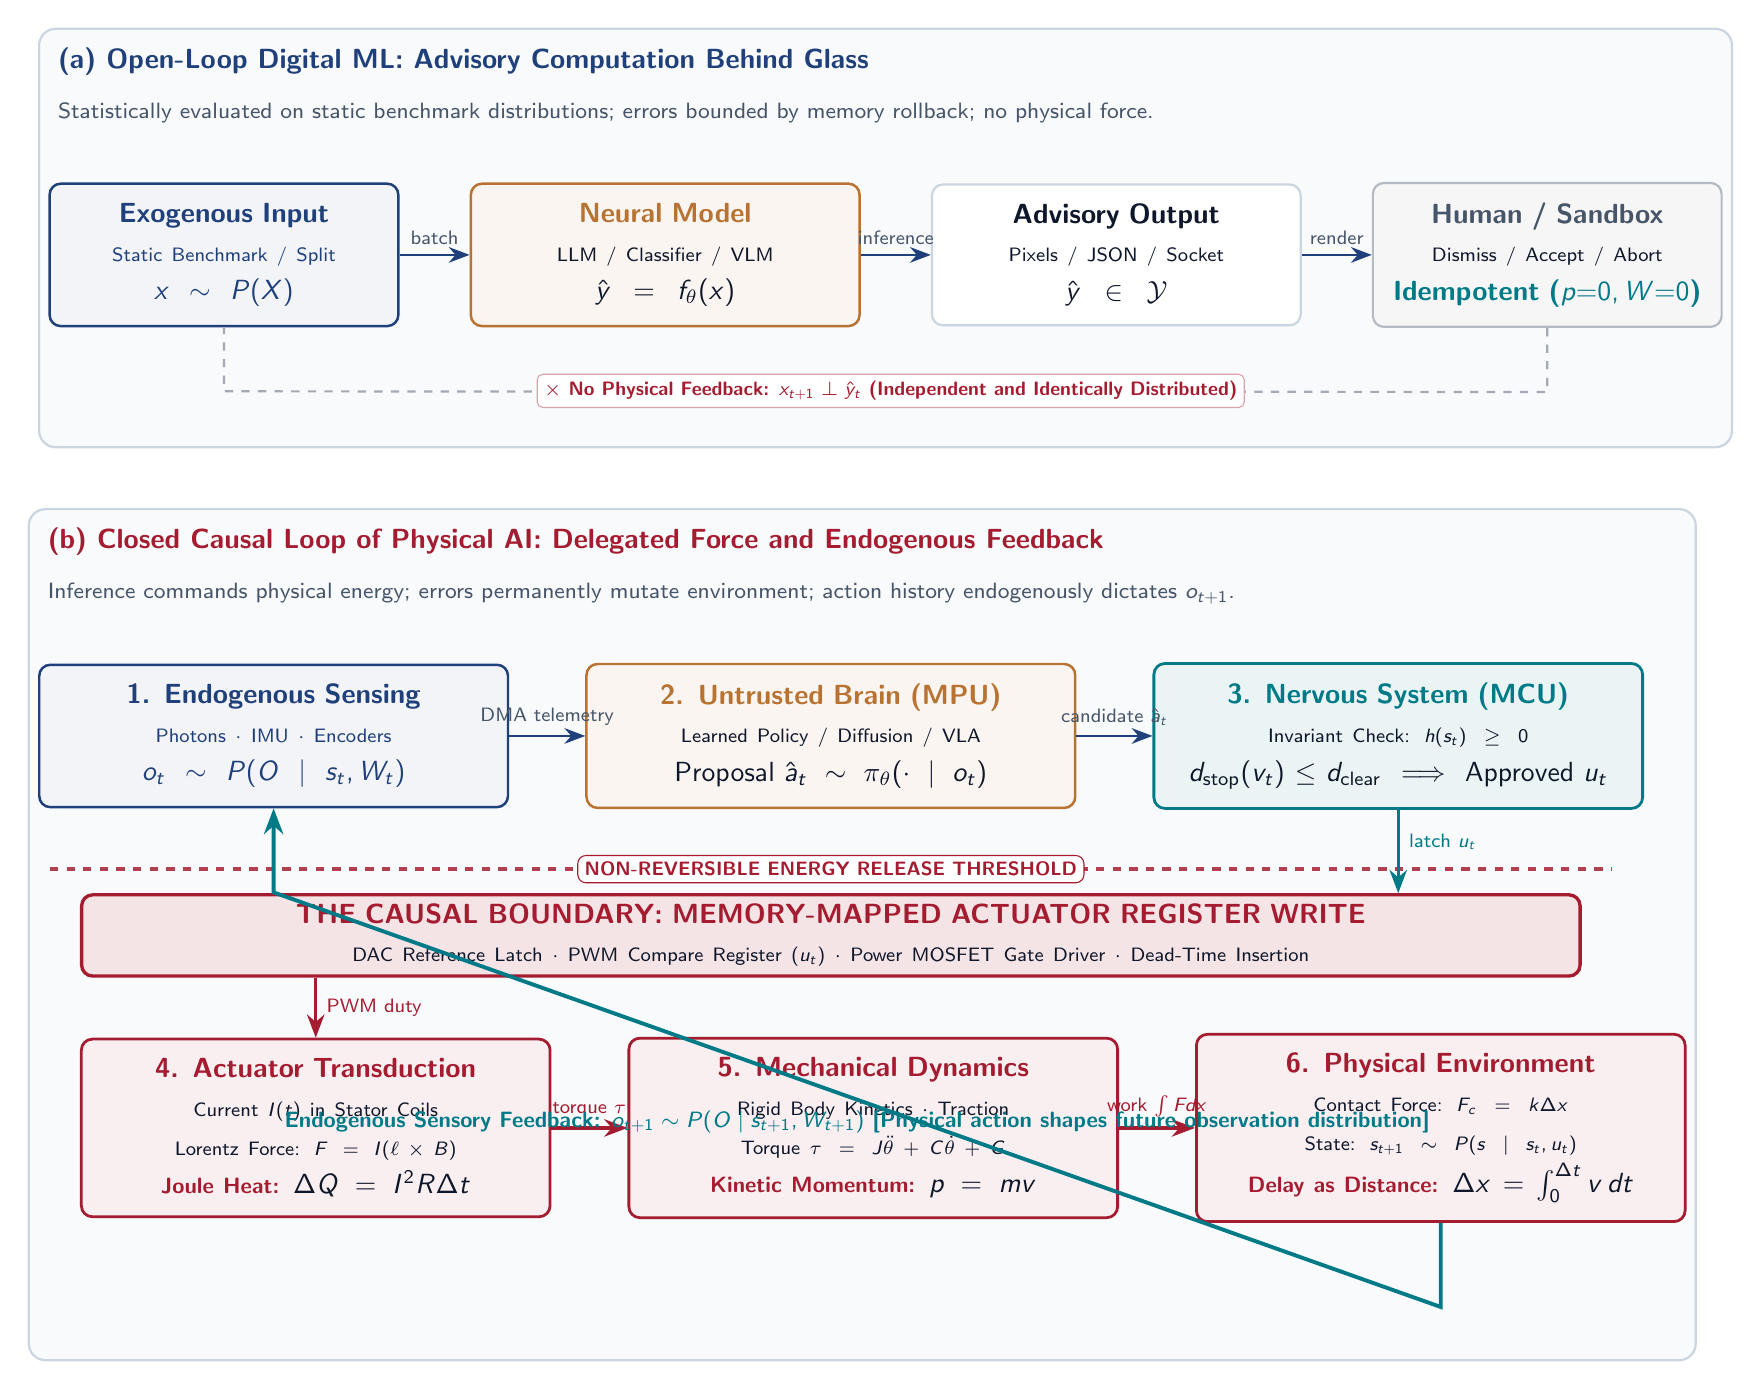
\begin{tikzpicture}[
  font=\sffamily,
  >=Stealth,
  box/.style={
    draw=cardborder,
    fill=cardbg,
    rounded corners=4pt,
    line width=0.8pt,
    inner sep=7pt,
    align=center,
    text=darkslate
  },
  databox/.style={
    draw=navy,
    fill=navy!6,
    rounded corners=4pt,
    line width=0.9pt,
    inner sep=7pt,
    align=center,
    text=navy
  },
  modelbox/.style={
    draw=bronze,
    fill=bronze!7,
    rounded corners=4pt,
    line width=0.9pt,
    inner sep=7pt,
    align=center,
    text=darkslate
  },
  gatebox/.style={
    draw=petrol,
    fill=petrol!8,
    rounded corners=4pt,
    line width=1.0pt,
    inner sep=7pt,
    align=center,
    text=darkslate
  },
  physbox/.style={
    draw=crimson,
    fill=crimson!7,
    rounded corners=4pt,
    line width=1.0pt,
    inner sep=7pt,
    align=center,
    text=darkslate
  },
  arr/.style={
    ->,
    line width=1.0pt,
    draw=navy
  },
  physarr/.style={
    ->,
    line width=1.2pt,
    draw=crimson
  },
  looparr/.style={
    ->,
    line width=1.2pt,
    draw=petrol
  },
  annot/.style={
    font=\sffamily\scriptsize,
    text=slate,
    align=center
  }
]

  % =========================================================================
  % PANEL (a): OPEN-LOOP DIGITAL ML (ADVISORY COMPUTATION BEHIND GLASS)
  % =========================================================================

  % Header Panel A
  \node[font=\sffamily\bfseries\normalsize, text=navy, anchor=north west] (titleA) at (0, 0) {
    (a) Open-Loop Digital ML: Advisory Computation Behind Glass
  };
  \node[font=\sffamily\footnotesize, text=slate, below=0.04in of titleA.south west, anchor=north west] (subA) {
    Statistically evaluated on static benchmark distributions; errors bounded by memory rollback; no physical force.
  };

  % Panel A Nodes
  \node[databox, text width=1.55in, below=0.25in of subA.south west, anchor=north west] (a_data) {
    \textbf{\color{navy} Exogenous Input}\\[2pt]
    {\scriptsize Static Benchmark / Split}\\[2pt]
    $x \sim P(X)$
  };

  \node[modelbox, text width=1.75in, right=0.35in of a_data] (a_model) {
    \textbf{\color{bronze} Neural Model}\\[2pt]
    {\scriptsize LLM / Classifier / VLM}\\[2pt]
    $\hat{y} = f_\theta(x)$
  };

  \node[box, text width=1.65in, right=0.35in of a_model] (a_out) {
    \textbf{\color{darkslate} Advisory Output}\\[2pt]
    {\scriptsize Pixels / JSON / Socket}\\[2pt]
    $\hat{y} \in \mathcal{Y}$
  };

  \node[box, draw=slate!40, fill=slate!5, text width=1.55in, right=0.35in of a_out] (a_env) {
    \textbf{\color{slate} Human / Sandbox}\\[2pt]
    {\scriptsize Dismiss / Accept / Abort}\\[2pt]
    {\color{petrol}\textbf{Idempotent ($p{=}0, W{=}0$)}}
  };

  % Panel A Connections
  \draw[arr] (a_data) -- node[above, annot] {batch} (a_model);
  \draw[arr] (a_model) -- node[above, annot] {inference} (a_out);
  \draw[arr] (a_out) -- node[above, annot] {render} (a_env);

  % Panel A Broken Feedback Annotation
  \coordinate (a_loop_drop) at ($(a_env.south) + (0, -0.32in)$);
  \coordinate (a_loop_left) at ($(a_data.south) + (0, -0.32in)$);
  \draw[dashed, line width=0.8pt, draw=slate!50] (a_env.south) -- (a_loop_drop) -- (a_loop_left) -- (a_data.south);
  
  \node[font=\sffamily\scriptsize\bfseries, text=crimson, fill=white, draw=crimson!40, rounded corners=2pt, inner sep=2.5pt] 
    at ($(a_model.south)!0.5!(a_out.south) + (0, -0.32in)$) (a_badge) {$\times$ No Physical Feedback: $x_{t+1} \perp \hat{y}_t$ (Independent and Identically Distributed)};

  \coordinate (a_bot) at ($(a_badge.south) + (0, -0.15in)$);

  % Background container for Panel A
  \begin{scope}[on background layer]
    \node[draw=cardborder, fill=subtlebg, rounded corners=6pt, line width=0.8pt,
          fit=(titleA) (subA) (a_data) (a_model) (a_out) (a_env) (a_bot)] (panelA_box) {};
  \end{scope}

  % =========================================================================
  % PANEL (b): CLOSED CAUSAL LOOP OF PHYSICAL AI (DELEGATED PHYSICAL FORCE)
  % =========================================================================

  % Header Panel B
  \node[font=\sffamily\bfseries\normalsize, text=crimson, below=0.35in of panelA_box.south west, anchor=north west] (titleB) {
    (b) Closed Causal Loop of Physical AI: Delegated Force and Endogenous Feedback
  };
  \node[font=\sffamily\footnotesize, text=slate, below=0.04in of titleB.south west, anchor=north west] (subB) {
    Inference commands physical energy; errors permanently mutate environment; action history endogenously dictates $o_{t+1}$.
  };

  % Row 1: Perception & Deliberation (matching full width)
  \node[databox, text width=2.15in, below=0.25in of subB.south west, anchor=north west] (b_sense) {
    \textbf{\color{navy} 1. Endogenous Sensing}\\[2pt]
    {\scriptsize Photons $\cdot$ IMU $\cdot$ Encoders}\\[2pt]
    $o_t \sim P(O \mid s_t, W_t)$
  };

  \node[modelbox, text width=2.25in, right=0.38in of b_sense] (b_brain) {
    \textbf{\color{bronze} 2. Untrusted Brain (MPU)}\\[2pt]
    {\scriptsize Learned Policy / Diffusion / VLA}\\[2pt]
    Proposal $\hat{a}_t \sim \pi_\theta(\cdot \mid o_t)$
  };

  \node[gatebox, text width=2.25in, right=0.38in of b_brain] (b_nervous) {
    \textbf{\color{petrol} 3. Nervous System (MCU)}\\[2pt]
    {\scriptsize Invariant Check: $h(s_t) \ge 0$}\\[2pt]
    $d_{\text{stop}}(v_t) \le d_{\text{clear}} \implies \text{Approved } u_t$
  };

  % The Causal Boundary Register (Center Transition Block)
  \node[draw=crimson, fill=crimson!12, rounded corners=4pt, line width=1.2pt, text width=7.4in, align=center,
        below=0.42in of b_brain.south, anchor=north] (b_register) {
    \textbf{\color{crimson} THE CAUSAL BOUNDARY: MEMORY-MAPPED ACTUATOR REGISTER WRITE}\\[2pt]
    {\scriptsize\color{darkslate} DAC Reference Latch $\cdot$ PWM Compare Register ($u_t$) $\cdot$ Power MOSFET Gate Driver $\cdot$ Dead-Time Insertion}
  };

  % Boundary Dashed Line and Badges
  \coordinate (cb_left) at ($(b_register.north west) + (-0.15in, 0.12in)$);
  \coordinate (cb_right) at ($(b_register.north east) + (0.15in, 0.12in)$);
  \draw[dashed, line width=1.3pt, crimson!85] (cb_left) -- (cb_right);
  \node[font=\sffamily\scriptsize\bfseries, fill=white, draw=crimson, rounded corners=3pt, inner sep=2.5pt, text=crimson]
    at ($(cb_left)!0.5!(cb_right)$) {NON-REVERSIBLE ENERGY RELEASE THRESHOLD};

  % Row 2: Physical Body & World Dynamics
  \node[physbox, text width=2.15in, below=0.30in of b_register.south west, anchor=north west] (b_act) {
    \textbf{\color{crimson} 4. Actuator Transduction}\\[2pt]
    {\scriptsize Current $I(t)$ in Stator Coils}\\[2pt]
    {\scriptsize Lorentz Force: $F = I (\ell \times B)$}\\[2pt]
    {\footnotesize\color{crimson}\textbf{Joule Heat:}} $\Delta Q = I^2 R \Delta t$
  };

  \node[physbox, text width=2.25in, right=0.38in of b_act] (b_body) {
    \textbf{\color{crimson} 5. Mechanical Dynamics}\\[2pt]
    {\scriptsize Rigid Body Kinetics $\cdot$ Traction}\\[2pt]
    {\scriptsize Torque $\tau = J \ddot{\theta} + C \dot{\theta} + G$}\\[2pt]
    {\footnotesize\color{crimson}\textbf{Kinetic Momentum:}} $p = m v$
  };

  \node[physbox, text width=2.25in, right=0.38in of b_body] (b_world) {
    \textbf{\color{crimson} 6. Physical Environment}\\[2pt]
    {\scriptsize Contact Force: $F_c = k \Delta x$}\\[2pt]
    {\scriptsize State: $s_{t+1} \sim P(s \mid s_t, u_t)$}\\[2pt]
    {\footnotesize\color{crimson}\textbf{Delay as Distance:}} $\Delta x = \int_0^{\Delta t} v \, dt$
  };

  % Panel B Dataflow Connections (Top Row)
  \draw[arr] (b_sense) -- node[above, annot] {DMA telemetry} (b_brain);
  \draw[arr] (b_brain) -- node[above, annot] {candidate $\hat{a}_t$} (b_nervous);

  % Connect Nervous System down to Register
  \draw[looparr, line width=1.2pt] (b_nervous.south) -- ++(0,-0.16in) -| node[pos=0.3, right, annot, text=petrol] {latch $u_t$} (b_register.north -| b_nervous.south);

  % Register down to Actuation
  \draw[physarr] (b_register.south -| b_act.north) -- node[right, annot, text=crimson] {PWM duty} (b_act.north);

  % Physical world connections (Left to Right)
  \draw[physarr] (b_act) -- node[above, annot, text=crimson] {torque $\tau$} (b_body);
  \draw[physarr] (b_body) -- node[above, annot, text=crimson] {work $\int F dx$} (b_world);

  % The Closed Causal Return Loop (Endogenous Observation)
  \coordinate (loop_drop) at ($(b_world.south) + (0, -0.42in)$);
  \coordinate (loop_left) at ($(b_sense.south) + (0, -0.42in)$);
  \draw[looparr, line width=1.4pt] (b_world.south) -- (loop_drop) 
    -- node[below, font=\sffamily\footnotesize\bfseries, text=petrol] {Endogenous Sensory Feedback: $o_{t+1} \sim P(O \mid s_{t+1}, W_{t+1})$ [Physical action shapes future observation distribution]} 
    (loop_left) -- (b_sense.south);

  \coordinate (b_bot) at ($(loop_drop) + (0, -0.22in)$);

  % Background container for Panel B
  \begin{scope}[on background layer]
    \node[draw=cardborder, fill=subtlebg, rounded corners=6pt, line width=0.8pt,
          fit=(titleB) (subB) (b_sense) (b_brain) (b_nervous) (b_register) (b_act) (b_body) (b_world) (b_bot)] (panelB_box) {};
  \end{scope}

\end{tikzpicture}
\end{document}
